\documentclass[dissertation.tex]{subfiles}
\begin{document}

\chapter[Optimal Biomarkers]{Identifying Optimal Biomarkers for Clinical Tests}
\label{chap:messina}


\emph{Thesis: Decision stump classifiers can be efficiently trained on high-throughput biomarker data, and provide a principled way to translate large multi-measurement research data into simple but high-performance clinical tests.}


\paragraph{Summary}


\section{Introduction}

Research and molecular pathology laboratories take strikingly different approaches to the measurement of biomarkers in patient samples.  Research work favours costly manual techniques, which quantify a large number of biomarkers in a relatively small number of samples.  Conversely, pathology laboratories make extensive use of highly automated turnkey systems, to robustly measure a relatively small number of biomarkers in a large number of samples.  In keeping with this divide, research and pathology laboratories often use very different technologies for the measurement of the same type of biomarker, such as RNA sequencing in research, and quantitative PCR in the clinical realm.  This difference in base technology complicates the translation of discoveries in research into application in the clinic.

Unfortunately, this difficult translation of research discoveries into clinical practice is absolutely necessary.  Although technologically not a perfect match, research and pathology techniques are complementary: biomarker \emph{discovery} requires research techniques capable of interrogating a huge number of potential biomarkers, but the \emph{application} of any discoveries needs pathology techniques that can reliably and economically handle a huge number of patient samples.  The two approaches are inseparable, and so finding effective ways to translate research findings into clinical application is critically important.  
* How can we get around this?
  - We can harmonise techniques.  Unfortunately, unlikely right now.
    OR...
  - We can find the best possible way to translate research -> clinical.

Effective clinical tests must satisfy a number of requirements, which can be used to guide the translation of a research finding into a clinical test.  Ideally, a clinical diagnostic or prognostic test should be based on the measurement of only a small number of biomarkers (###).  Additionally, it should be highly robust to technical effects, and the inevitable variation in sample quality and handling that comes with clinical specimens (###).  The results of most tests will be interpreted as a simple binary outcome, and the optimal detection performance of this binary variable will vary depending on the particular clinical application (###).  Taking all these requirements into account, a technique to translate discovery biomarker measurements into a clinical test should identify a single biomarker that, when its level is thresholded, yields a particular class separation performance with maximal robustness.

* Existing methods do not do this.
* Consider common ML algos.  They all benefit from many features (eg. SVM, PAM, RF).
* Feature selection can be used to reduce feature count, obviously.
* However, what we need is:
  A Cutting down all the way to just one feature
  B With defined separation performance
  C At maximal robustness.
* There's nothing really out there to achieve that, because A is featsel, but B,C are class, and B is cost-sensitive.
* There *is* evidence that it is possible.  Cue small classifier papers.

* Enter Messina.  Single-feature cost-sensitive maximum-margin classifiers.
* Maximum margin -> robustness (Vapnik)
* Messina paper.
* Messina in lit., comparisons.
* Hook to limitations

* Messina2 addresses limitations in 1.
  - More general objective function
  - Makes it possible to do prognostics as well

* Ok, now chapter outline:
  1) Messina
  2) Messina2
  3) Simulation Experiments:
     A) Margin => Perf robustness.  Two expts: symbolic on class, simul on surv.
     B) Messina2 class better than competing approaches.
     C) Messina2 surv better than competing approaches.
  4) Application example: MessinaSurv on APGI to find better biomarker leads.
  5) Discussion
  6) Methods (for sims only -- cover algos in 1 & 2)


A core task in bioinformatics is identifying biomolecules that are differentially-expressed between experimental groups. When groups are homogeneous sets of replicates, all identical except for random measurement noise, the detection of differential expression is effectively addressed by techniques based in classical statistics.  Unfortunately, this ideal laboratory situation rarely exists in clinical samples, such as the tumour samples collected as part of large-scale observational studies like the ICGC and TCGA.

The expression levels of biomolecules within clinical samples may vary widely within sample groups due to many factors, such as the presence of latent biological subtypes, different stages of disease, environmental factors, and a range of technical effects. The net result of this heterogeneity is increased within-group variance, leading to a reduction in the power of classical techniques to detect differential expression. Importantly, this reduction in power is strongest for biomolecules with the most intra-group expression variance. The levels of such high-variance molecules potentially reflect latent biological subtypes, and thus they are of great interest, yet are the most likely to be ignored by classical differential expression detection techniques. Consequently, a real need exists for methods to reliably identify differential expression in complex and poorly-controlled observational data, such as those generated by current disease genomics efforts.

Recently, a number of techniques have been reported for the identification of differential expression in the presence of outlier samples and expression heterogeneity (for overviews see for example Karrila et al. (2011) and Bottomly et al. (2013)). Of these, the Messina algorithm (Pinese et al., 2009) is unique in that it is tunable, allowing the user to smoothly trade robustness to outliers against sensitivity to subtle changes in expression. In the presence of outliers, Messina outperformed limma (Smyth, 2004) for the detection of differential expression, and has been recommended for this purpose in an independent comparison of existing methods (Karrila et al., 2011). However, Messina is only available as a standalone program, reducing its utility in bioinformatic pipelines, and, in common with other outlier-aware techniques, cannot identify biomolecules associated with outcome.

Here we present Messina2, an enhanced version of Messina that is implemented as the ‘messina’ R package, available in Bioconductor versions 2.14 and above. It contains all the original functionality of Messina, with the additional unique capability to identify biomolecules associated with a censored outcome variable. In the following we describe the Messina2 algorithm and demonstrate its application with case studies.

There are things on prognostic biomarkers that really should be here. Stuff on the ad-hoc nature of current approaches (eg. median split, or cutpoint optimization), and the general unsuitability of stats-based approaches (eg. Cox) for the generation of a good biomarker. There’s also the more general problem of cardinality – most of the prognostic biomarker stuff out there is based on large signatures, because that’s a way to get a good split from the kind of genes found by current methods. There’s very little on good ways to choose single-gene biomarkers. No room for all of that, though!

marcow’s idea for some intro text:``Two of the most common analytical scenarios for clinical samples are classification and survival; the former has been addressed by a number of methods, including Messina, in the context of heterogeneity, as reviewed by refs. Survival in the presence of heterogeneity remains largely unsolved. Here we extend Messina to solve
survival in the context of hereogeneity and additionally extend the capabilities of the original Messina algorithm via R''

http://en.wikipedia.org/wiki/NanoString_Technologies
http://en.wikipedia.org/wiki/Oncotype_DX_Colon_Cancer_Assay
http://en.wikipedia.org/wiki/Oncotype_DX
http://en.wikipedia.org/wiki/MammaPrint
http://en.wikipedia.org/wiki/Symphony_(Agendia)
http://www.agendia.com/healthcare-professionals/colon-cancer/
http://www.agendia.com/healthcare-professionals/breast-cancer/mammaprint/


TODO: mention the preponderance of biomarkers that never get used?  Sigs. especially!

A number of factors contribute to the divide in methodology between research and clinical laboratories.  Relative to clinical tests, research techniques are labour-intensive, costly, likely less robust, and have low sample throughput.  Being research methods, they are also not offered by manufacturers as validated and complete turnkey tests, and so require extensive work on in-house development and certification.  These elements, combined with the noted inertia in the medical profession for adopting new techniques, combine to make bespoke and complex research-grade methods 

* Inertia -- complex cert. process, doc uptake slow.
* Development -- no turn-key solns.  Ties in with cert issues.
* Cost -- much higher for research methods.  Also buy-in cost.
* Scalability -- disc. methods are low n, high p.  Path. are high n, low p.


\section{Results}

\section{Discussion}

\section{Methods}



"How can we select markers that have the best possible chances of making it in the clinic?"


The Messina chapter.  What is this all about?  Selecting biomolecules.  For what purpose?  Differently how?  What makes this special?

OK back up.  Let's go back to basics.  Consider this situation.  There is a need to develop a diagnostic or prognostic test, for clinical application.  What requirements does this test have?
  * High performance
    - But notably, performance can be nuanced, not simply correct -- perhaps some errors are preferable to others.
  * Robustness (ie. performance is good, even in the face of:
    - cohort differences
    - technical differences (eg inter-lab)
    - sample handling differences (eg degradation, alternate storage or processing, sample age)
  * Ease of use
    - measures a small number of variables, as small as possible.
  * Translatability (can be easily moved to a clinical setting)
    - measures a small number of variables
    - uses existing technologies, as much as possible

Rolling all these together, it means we basically need an IHC- or ELISA-based measurement, on as few biomarkers as possible.  Just one would be ideal.

So what do we know about IHC?
  * It's very nonlinear
  * It's protein level based
  * There can be significant differences between labs, due to tissue processing, AR, and staining.  The latter two are less serious for clinical-grade stuff, but tissue processing is still a problem.  Time before fixation, conditions before fixation, time in fixative, type of fixative, conditions of embedding, time in storage in paraffin.
  * There can be differences between pathologists re: scoring.

What we get from this is that we need a very robust marker.  If we only have mRNA levels, then for starters the mRNA-protein correlation is only approximate.  We want to stack the deck in our favour as much as we can, by choosing mRNAs with huge gaps between the expression levels of interest.  Even if we have protein, all the other aspects again reinforce the need for a high-margin feature.  The bigger the margin, the bigger the likely robustness to all the various sources of error.

Remember this is not a proof or guarantee that a given marker will make a good test.  It's rather an answer to the question: "How can we select markers that have the best possible chances of making it in the clinic?"


Relevant literature ideas:
  * That reference on cutpoint searching => high FDR
  * Something about margins and performance?  Surely Vaponik's early stuff will cover this.

Bad practice:
  * Median cut:
    * Examples of use:
      - http://www.biomedcentral.com/1756-0500/7/546
      - http://breast-cancer-research.com/content/12/5/r85
  * "Optimal" cut: 
    * Examples of use: 
      - http://clincancerres.aacrjournals.org/content/10/21/7252.full
      - http://journals.plos.org/plosone/article?id=10.1371/journal.pone.0051862
    * Statistical corrections:
      - http://www.mayo.edu/research/documents/biostat-79pdf/doc-10027230   (also lots of useful refs here)
      - https://books.google.com.au/books?id=KSq0e-6VFJ0C&pg=PA273&lpg=PA273&dq=log+rank+cut+points&source=bl&ots=0c07185Yb1&sig=Y7g8m9U0LHepQr1FxjrJzE0_rv8&hl=en&sa=X&ei=Lj_6VJII1OPwBY7ZgZgE&ved=0CEEQ6AEwBg#v=onepage&q=log%20rank%20cut%20points&f=false
      - https://www.fdm.uni-freiburg.de/publications-preprints/preprints/papers/pre73.pdf
      - https://books.google.com.au/books?id=C753uzZztPAC&pg=PA423&lpg=PA423&dq=log+rank+optimal+cut+points&source=bl&ots=__ay7uRwZ4&sig=e4IF1oKV71mw8XYU5qUiSl7JQ3g&hl=en&sa=X&ei=1z_6VOu1CImG8QW4o4LQAw&ved=0CFcQ6AEwCA#v=onepage&q=log%20rank%20optimal%20cut%20points&f=false
      - But note that these generally only correct P-values, and *do not* correct for overestimation (inflation) of differences.
    * Issues: 
      - http://europepmc.org/backend/ptpmcrender.fcgi?accid=PMC2063091&blobtype=pdf
      -~\cite{Altman1994}


\begin{algorithm}
  \KwData{An $n$-tuple of covariate measurements $x$, an $n$-tuple of associated dependent values $y$, a $m$-vector of candidate cutpoints $c$, and an objective function $f: (\mathbb{B}^n, \mathbb{Y}^n) \rightarrow \mathbb{B}$.  $x$ and $c$ are to be in ascending order.  The domain of $y$ is given as $\mathbb{Y}^n$, as it varies between modes of Messina.}
  \KwResult{If the fit failed, $\varnothing$.  Otherwise, a tuple of two real values: (optimal classifier threshold, resultant classifier margin).}

  \Begin {
	\tcp{Evaluate the objective $f$ on each threshold in $c$}
	\For{$i \leftarrow 1$ \KwTo $m$}{
		$o^+_i \longleftarrow f\left(\left[~\left[x_j \geq c_i\right]~\right]_{j=1}^n, y\right)$\;
		$o^-_i \longleftarrow f\left(\left[~\left[x_j < c_i\right]~\right]_{j=1}^n, y\right)$\;
	}
	
	\tcp{If no threshold passed $f$, return $\varnothing$}
	\If{$o^+ \vee o^-$ is all $\mathrm{false}$}{
      \KwRet $\varnothing$\;
    }
	
	\tcp{Search $o^+$ and $o^-$ for the widest margin contiguous interval that passes $f$}
	$(t^+, \Delta^+) \longleftarrow$ BestInterval$\left(o^+, c\right)$\;
	$(t^-, \Delta^-) \longleftarrow$ BestInterval$\left(o^-, c\right)$\;
	
	\tcp{Return the best of the $o^+$ and $o^-$ results}
	\eIf{$\Delta^+ \geq \Delta^-$}{
	  \KwRet{$(t^+, \Delta^+)$}\;
	}{
	  \KwRet{$(t^-, \Delta^-)$}\;
	}
  }
  \label{alg:mess_messina1}
  \caption{Messina1}
\end{algorithm}


\begin{algorithm}
  \KwData{An $n$-tuple of covariate measurements $x$, and a minimum subclass fraction $b$.  $x$ is to be sorted in ascending order.}
  \KwResult{A tuple of candidate cutpoints $c$, with values sorted in ascending order.}

  \Begin {
  	$x' \longleftarrow \mbox{unique}(x)$\;
  	\For{$i \leftarrow 1$ \KwTo $\vert x' \vert - 1$}{
  		$p \longleftarrow \frac{1}{2} \left({x'}_i + {x'}_{i+1}\right)$\;
  		$s \longleftarrow \frac{1}{n} \sum_{i=1}^n \left[ x_i < p \right] $\;
  		\If{$s \geq b \wedge s \leq 1-b$}{
	  		$c \longleftarrow c \oplus p$\;
	  	}
  	}
  	\If{$b = 0$}{
	  	$c \longleftarrow -\infty \oplus c \oplus \infty$\;
	}
  	
	\KwRet{$c$}\;
  }
  \label{alg:mess_cutpoints}
  \caption{MakeCutpoints}
\end{algorithm}


\begin{algorithm}
  \KwData{An $n$-tuple of covariate measurements $x$, an $n$-tuple of associated dependent values $y$, an objective function $f: (\mathbb{B}^n, \mathbb{Y}^n) \rightarrow \mathbb{B}$, a minimum subclass fraction $b$, and a number of bootstrap rounds $r$.  $x$ is to be sorted in ascending order.  The domain of $y$ is given as $\mathbb{Y}^n$, as it varies between modes of Messina.}
  \KwResult{If the fit failed, $\varnothing$.  Otherwise, a tuple of two real values: (optimal classifier threshold, resultant classifier margin).}

  \Begin {
  	$n_pass \longleftarrow 0$\;
  	\For{$i \leftarrow 1$ \KwTo $r$}{
  		\tcp{Generate a bootstrap sample of (x, y)}
  		$(x_in, y_in, x_out, y_out) \longleftarrow \mbox{BootstrapResample}\left( x, y \right)$\;
  		
  		\tcp{Train MessinaCore on this bootstrap sample}
  		$(t_in, d_in, \Delta_in) \longleftarrow \mbox{MessinaCore}\left( x_in, y_in, b, f \right)$\;
  		
  		\tcp{Assess performance of the MessinaCore classifier on the out-of-bag samples}
  		\If{$d_in \neq 0$}{
  			\If {$\longleftarrow f\left(\left[~\left[ x_{out_j} d_in \geq t_in d_in\right]~\right]_{j=1}^{\vert x_out \vert}, y_out\right)$\;}{
  				$n_pass \longleftarrow n_pass + 1$\;
  			}
  		}
  	}
  	
  	\tcp{Did the in-bag trained classifiers satisfy out-of-bag performance requirements in at least half of the bootstrap rounds?}
  	\eIf{$n_pass \geq \frac{1}{2}r$}{
	  	\tcp{Yes; return the fit on the full data}
  		\KwRet{$\mbox{MessinaCore}\left( x, y, b, f \right)$}\;
  	}{
  		\tcp{No; this fit failed.}
  		\KwRet{$\varnothing$}\;
	}
  }
  \label{alg:mess_messina2}
  \caption{Messina2}
\end{algorithm}


\begin{algorithm}
  \KwData{An $n$-tuple of covariate measurements $x$, an $n$-tuple of associated dependent values $y$, a minimum subclass fraction $b$, and an objective function $f: (\mathbb{B}^n, \mathbb{Y}^n) \rightarrow \mathbb{B}$.  $x$ and $c$ are to be in ascending order.  The domain of $y$ is given as $\mathbb{Y}^n$, as it varies between modes of Messina.}
  \KwResult{A tuple of three values.  If the fit failed, $(0, 0, 0)$.  If the fit succeeded, (optimal classifier threshold, optimal classifier direction, resultant classifier margin).}

  \Begin {
  	\tcp{Define candidate thresholds $c$ as the midpoints between consecutive unique values of $x$}
  	$c \longleftarrow \mbox{MakeCutpoints}\left(x, b\right)$\;
  	$m \longleftarrow \vert c \vert$\;
  
	\tcp{Evaluate the objective $f$ on each threshold in $c$}
	\For{$i \leftarrow 1$ \KwTo $m$}{
		$o^+_i \longleftarrow f\left(\left[~\left[x_j \geq c_i\right]~\right]_{j=1}^n, y\right)$\;
		$o^-_i \longleftarrow f\left(\left[~\left[x_j < c_i\right]~\right]_{j=1}^n, y\right)$\;
	}
	
	\tcp{If no threshold passed $f$, return $\varnothing$}
	\If{$o^+ \vee o^-$ is all $\mathrm{false}$}{
      \KwRet $\varnothing$\;
    }
	
	\tcp{Search $o^+$ and $o^-$ for the widest margin contiguous interval that passes $f$}
	$(t^+, \Delta^+) \longleftarrow$ BestInterval$\left(o^+, c\right)$\;
	$(t^-, \Delta^-) \longleftarrow$ BestInterval$\left(o^-, c\right)$\;
	
	\tcp{Return the best of the $o^+$ and $o^-$ results}
	\eIf{$\Delta^+ \geq \Delta^-$}{
	  \KwRet{$(t^+, +1, \Delta^+)$}\;
	}{
	  \KwRet{$(t^-, -1, \Delta^-)$}\;
	}
  }
  \label{alg:mess_core}
  \caption{MessinaCore}
\end{algorithm}


\begin{algorithm}
  \KwData{$o \in \mathbf{B}^m$, $c \in \mathbf{R}^m$, $x \in \mathbf{R}^n$}
  \KwResult{$(c^* \in \mathbf{R}, \Delta^* \in [0, \infty))$}

  \Begin {
    $\Delta^* \longleftarrow 0$\;
    $c^* \longleftarrow 0$\;
    
    $i \longleftarrow 1$\;
    \While{$i \leq m$}{
      \If{$o_i$ is $\mathrm{true}$}{
        $r_L \longleftarrow \sup \{x_k~|~x_k \leq c_i \wedge k \in \mathbb{N}^+ \wedge k \leq n \}$\;
        \For{$j \leftarrow i$ \KwTo $m$}{
          \eIf{$o_j$ is $\mathrm{true}$}{
            $r_R \longleftarrow \sup \{x_k~|~x_k \leq c_j \wedge k \in \mathbb{N}^+ \wedge k \leq n \}$\;
          }{
            break\;
          }
        }

		$\Delta \longleftarrow r_R - r_L$\;
        \If{$\Delta > \Delta^*$}{
          $\Delta^* \longleftarrow \Delta$\;
          $c^* \longleftarrow r_L + \frac{1}{2}\Delta$\;
        }
        
        $i \longleftarrow j$\;
      }
      $i \longleftarrow i + 1$\;
    }
    \KwRet{$(c^*, \Delta^*)$}\;
  }
  
  \label{alg:mess_bestinterval}
  \caption{BestInterval}
\end{algorithm}


\begin{align*}
f_M(s, y) &= \left[ p_n \geq l_n \wedge p_c \geq l_c \right] \\
p_n &= \frac{\sum_i{\left[ s_i \wedge y_i \right]}}{\sum_i{\left[ y_i \right]}} \\
p_c &= \frac{\sum_i{\left[ \neg s_i \wedge \neg y_i \right]}}{\sum_i{\left[ \neg y_i \right]}} \\
\end{align*}
\begin{align*}
f_C(s, y) &= \left[ p_f \geq l_f \right] \\
p_f &= TODO \\
\end{align*}
\begin{align*}
f_{\tau}(s, y) &= \left[ p_\tau \geq l_\tau \right] \\
p_\tau &= \frac{\tau_c + \frac{1}{2}\tau_t}{\tau_c + \tau_d + \tau_t} \\
\tau_c &= \sum_i^n{\sum_{j=i+1}^n{\left[\tau_v_i \wedge \neg \left(s_i = s_j \vee y_{t,i} = y_{t,j}\right) \wedge s_i = 1 \right]}} \\
\tau_d &= \sum_i^n{\sum_{j=i+1}^n{\left[\tau_v_i \wedge \neg \left(s_i = s_j \vee y_{t,i} = y_{t,j}\right) \wedge s_i = 0 \right]}} \\
\tau_t &= \sum_i^n{\sum_{j=i+1}^n{\left[\tau_v_i \wedge \left(s_i = s_j \vee y_{t,i} = y_{t,j}\right)\right]}} \\
\tau_v_i &= \left(y_{e,i} = 1 \vee y_{e,j} = 1\right) \wedge \left(y_{t,i} \geq y_{t,j} \vee y_{e,i} = 1 \right) 
\end{align*}
\begin{align*}
f_{\tau'}(s, y) &= \left[ p_\tau' \geq l_\tau' \right] \\
p_{\tau'} &= \frac{\tau_c}{\tau_c + \tau_d}
\end{align*}

\begin{figure}
\centering
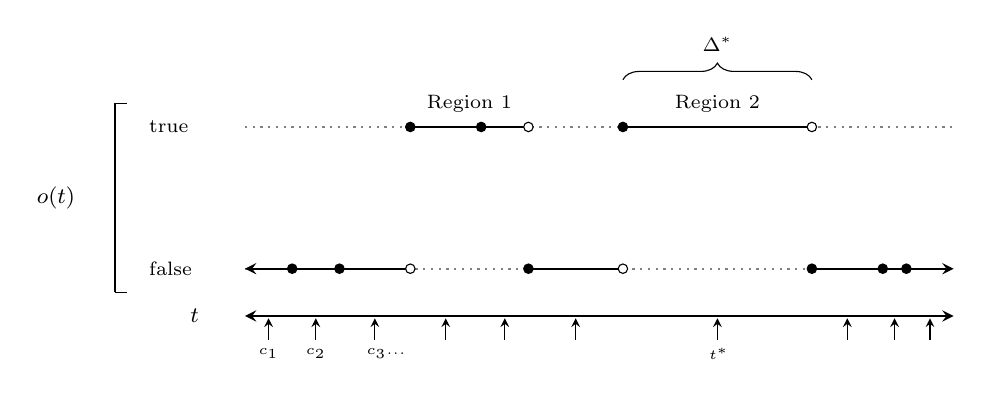
\begin{tikzpicture}[
    axis/.style={thick,<->,>=stealth},
    guide/.style={thick,dotted,gray},
    graphline/.style={thick,black},
    threshmark/.style={thin,->,>=stealth}]

  \def\f{*0.6}

  \draw[axis]
    (1\f,2\f) -- (16\f,2\f);

  \draw[guide]
    (1\f,3\f) -- (16\f,3\f)
    (1\f,6\f) -- (16\f,6\f);

  \draw[graphline,<-,>=stealth]
    (1\f,3\f) -- (4.5\f,3\f);
  \draw[graphline,->,>=stealth]
    (13\f,3\f) -- (16\f,3\f);
  \draw[graphline]
    (4.5\f,6\f) -- (7\f,6\f)
    (7\f,3\f) -- (9\f,3\f)
    (9\f,6\f) -- (13\f,6\f);

  \filldraw[black,draw=black] (2\f,3\f) circle [radius=0.1\f];
  \filldraw[black,draw=black] (3\f,3\f) circle [radius=0.1\f];
  \filldraw[black,draw=black] (4.5\f,6\f) circle [radius=0.1\f];
  \filldraw[black,draw=black] (6\f,6\f) circle [radius=0.1\f];
  \filldraw[black,draw=black] (7\f,3\f) circle [radius=0.1\f];
  \filldraw[black,draw=black] (9\f,6\f) circle [radius=0.1\f];
  \filldraw[black,draw=black] (13\f,3\f) circle [radius=0.1\f];
  \filldraw[black,draw=black] (14.5\f,3\f) circle [radius=0.1\f];
  \filldraw[black,draw=black] (15\f,3\f) circle [radius=0.1\f];
  \filldraw[white,draw=black] (4.5\f,3\f) circle [radius=0.1\f];
  \filldraw[white,draw=black] (7\f,6\f) circle [radius=0.1\f];
  \filldraw[white,draw=black] (9\f,3\f) circle [radius=0.1\f];
  \filldraw[white,draw=black] (13\f,6\f) circle [radius=0.1\f];

%  \draw[threshmark] (1.5\f,3.5\f) -- (1.5\f,3.05\f);
%  \draw[threshmark] (2.5\f,3.5\f) -- (2.5\f,3.05\f);
%  \draw[threshmark] (3.75\f,3.5\f) -- (3.75\f,3.05\f);
%  \draw[threshmark] (5.25\f,6.5\f) -- (5.25\f,6.05\f);
%  \draw[threshmark] (6.5\f,6.5\f) -- (6.5\f,6.05\f);
%  \draw[threshmark] (8\f,3.5\f) -- (8\f,3.05\f);
%  \draw[threshmark] (11\f,6.5\f) -- (11\f,6.05\f);
%  \draw[threshmark] (13.75\f,3.5\f) -- (13.75\f,3.05\f);
%  \draw[threshmark] (14.75\f,3.5\f) -- (14.75\f,3.05\f);
%  \draw[threshmark] (15.5\f,3.5\f) -- (15.5\f,3.05\f);
  
%  \node[align=left] at (1.5\f,3.8\f) {\tiny $o_1$};
%  \node[align=left] at (2.5\f,3.8\f) {\tiny $o_2$};
%  \node[align=left] at (3.75\f,3.8\f) {\tiny $o_3$};
%  \node[align=left,text width=10\f] at (5.25\f,6.8\f) {\tiny $o_4...$};

  \draw[threshmark] (1.5\f,1.5\f) -- (1.5\f,1.95\f);
  \draw[threshmark] (2.5\f,1.5\f) -- (2.5\f,1.95\f);
  \draw[threshmark] (3.75\f,1.5\f) -- (3.75\f,1.95\f);
  \draw[threshmark] (5.25\f,1.5\f) -- (5.25\f,1.95\f);
  \draw[threshmark] (6.5\f,1.5\f) -- (6.5\f,1.95\f);
  \draw[threshmark] (8\f,1.5\f) -- (8\f,1.95\f);
  \draw[threshmark] (11\f,1.5\f) -- (11\f,1.95\f);
  \draw[threshmark] (13.75\f,1.5\f) -- (13.75\f,1.95\f);
  \draw[threshmark] (14.75\f,1.5\f) -- (14.75\f,1.95\f);
  \draw[threshmark] (15.5\f,1.5\f) -- (15.5\f,1.95\f);

  \node[align=left] at (1.5\f,1.2\f) {\tiny $c_1$};
  \node[align=left] at (2.5\f,1.2\f) {\tiny $c_2$};
  \node[align=left,text width=10\f] at (3.75\f,1.2\f) {\tiny $c_3...$};
%  \node[align=left] at (3.75\f,1.2\f) {\tiny $c_3$};
%  \node[align=left,text width=10\f] at (5.25\f,1.2\f) {\tiny $c_4...$};
  \node[align=left,text width=10\f] at (11\f,1.2\f) {\tiny $t^*$};

  \node[align=right,text width=30\f] at (-0.5\f,2\f) {\footnotesize $t$};
  \node[align=left,text width=30\f] at (-0.5\f,3\f) {\scriptsize false};
  \node[align=left,text width=30\f] at (-0.5\f,6\f) {\scriptsize true};

  \draw 
    (-1.5\f,2.5\f) -- (-1.75\f,2.5\f)
    (-1.75\f,2.5\f) -- (-1.75\f,6.5\f)
    (-1.5\f,6.5\f) -- (-1.75\f,6.5\f);

  \node at (-3\f,4.5\f) {\footnotesize $o(t)$};

%  \draw[decorate,decoration={brace,amplitude=10\f},rotate=0] (4.5\f,7\f) -- (7\f,7\f);
  \draw[decorate,decoration={brace,amplitude=10\f},rotate=0] (9\f,7\f) -- (13\f,7\f);

  \node[align=center] at (5.75\f,6.5\f) {\scriptsize Region 1};
  \node[align=center] at (11\f,6.5\f) {\scriptsize Region 2};
  \node[align=center] at (11\f,7.75\f) {\scriptsize $\Delta^*$};
\end{tikzpicture}
\caption[The BestInterval algorithm]{Operation of the BestInterval algorithm.  Example values of a binary objective function $o(t)$ are shown for a range of input thresholds $t$.  At discrete points defined by observed data values (shown as dots), this objective function can transition, as an observed data point changes its value relative to $t$, and therefore its assigned class.  Two regions in which $o(t) = \mbox{true}$ are shown.  BestInterval locates all such regions, selects the one with largest measure on $t$ (margin), and returns its centre and margin as $(t^*, \Delta^*)$.  In this example, the centre and margin of region 2 would be returned.  To ensure that $o(t)$ is sampled at sufficient density, candidate thresholds $c_1, c_2, \dots$ are defined between all consecutive values, and beyond the extrema, of $x$; these are indicated by small arrows.  Each $c_i$ is associated with an $o_i$, as $o_i = o(c_i)$.}
\label{fig:mess_bestinterval}
\end{figure}

\end{document}
